%% 
%% Copyright 2007-2025 Elsevier Ltd
%% 
%% This file is part of the 'Elsarticle Bundle'.
%% ---------------------------------------------
%% 
%% It may be distributed under the conditions of the LaTeX Project Public
%% License, either version 1.3 of this license or (at your option) any
%% later version.  The latest version of this license is in
%%    http://www.latex-project.org/lppl.txt
%% and version 1.3 or later is part of all distributions of LaTeX
%% version 1999/12/01 or later.
%% 
%% The list of all files belonging to the 'Elsarticle Bundle' is
%% given in the file `manifest.txt'.
%% 
%% Template article for Elsevier's document class `elsarticle'
%% with numbered style bibliographic references
%% SP 2008/03/01
%% $Id: elsarticle-template-num.tex 272 2025-01-09 17:36:26Z rishi $
%%
% \documentclass[preprint,12pt]{elsarticle}

%% Use the option review to obtain double line spacing
%% \documentclass[authoryear,preprint,review,12pt]{elsarticle}

%% Use the options 1p,twocolumn; 3p; 3p,twocolumn; 5p; or 5p,twocolumn
%% for a journal layout:
%% \documentclass[final,1p,times]{elsarticle}
% \documentclass[final,1p,times,twocolumn]{elsarticle}
%% \documentclass[final,3p,times]{elsarticle}
% \documentclass[final,3p,times,twocolumn]{elsarticle}
% \documentclass[final,5p,times]{elsarticle}
\documentclass[final,5p,times,twocolumn]{elsarticle}

%% For including figures, graphicx.sty has been loaded in
%% elsarticle.cls. If you prefer to use the old commands
%% please give \usepackage{epsfig}

%% The amssymb package provides various useful mathematical symbols
\usepackage{amssymb}
%% The amsmath package provides various useful equation environments.
\usepackage{amsmath}
%% The amsthm package provides extended theorem environments
% \usepackage{amsthm}

%% Load algorithm2e
\usepackage{algorithm2e}
\RestyleAlgo{ruled}

%% Tikz
\usepackage{tikz}

%% The lineno packages adds line numbers. Start line numbering with
%% \begin{linenumbers}, end it with \end{linenumbers}. Or switch it on
%% for the whole article with \linenumbers.
%% \usepackage{lineno}

% \journal{}

\begin{document}

\begin{frontmatter}

%% Title, authors and addresses

%% use the tnoteref command within \title for footnotes;
%% use the tnotetext command for theassociated footnote;
%% use the fnref command within \author or \affiliation for footnotes;
%% use the fntext command for theassociated footnote;
%% use the corref command within \author for corresponding author footnotes;
%% use the cortext command for theassociated footnote;
%% use the ead command for the email address,
%% and the form \ead[url] for the home page:
%% \title{Title\tnoteref{label1}}
%% \tnotetext[label1]{}
%% \author{Name\corref{cor1}\fnref{label2}}
%% \ead{email address}
%% \ead[url]{home page}
%% \fntext[label2]{}
%% \cortext[cor1]{}
%% \affiliation{organization={},
%%             addressline={},
%%             city={},
%%             postcode={},
%%             state={},
%%             country={}}
%% \fntext[label3]{}

\title{Implementation and Validation of 1D Return Mapping 
Algorithms for Plasticity and Viscoplasticity}

%% use optional labels to link authors explicitly to addresses:
%% \author[label1,label2]{}
%% \affiliation[label1]{organization={},
%%             addressline={},
%%             city={},
%%             postcode={},
%%             state={},
%%             country={}}
%%
%% \affiliation[label2]{organization={},
%%             addressline={},
%%             city={},
%%             postcode={},
%%             state={},
%%             country={}}

\author{Billy Guy} %% Author name

%% Author affiliation
\affiliation{
  % organization={},%Department and Organization
            % addressline={}, 
            % city={},
            % postcode={}, 
            state={Québec},
            country={Canada}}

%% Abstract
\begin{abstract}
%% 1. General Background
%% 2. Specific background
%% 3. Problem statement
%% 4. Here we show...
%% 5. Approach and results
%% 6. Implications

%% Text of abstract
Constitutive material models are the cornerstone of finite element analysis in solid mechanics. Material behavior direct consequences on how displacements, velocities and accelerations are calculated at the nodes of each elements. For viscoplastic behavior, mathematical definitions ties the evolution of the viscoplastic strain to the evolution of stresses and strain over time. Thus for each increment of strain and time, algorithm must find the equilibrium at wich Karush-Kuhn-Tucker (KKT) conditions are met. However, since viscoplastic material exhibit stress dissipation, these conditions needs to be relaxed to accomodate the accumulation of viscoplastic strain. In this mock paper, a return mapping algorithm for the Perzyna viscoplastic model will be implemented to solve for the equilibrium of the KKT conditions considering the overstress concepts. The basic definitions of return mapping for regular plasticity will be showed and will serve as a basis for further implementation of the Perzyna model to show the impact of strain rates and material properties on constitutive behavior.
\end{abstract}

% %%Graphical abstract
% \begin{graphicalabstract}
% %\includegraphics{grabs}
% \end{graphicalabstract}

% %%Research highlights
% \begin{highlights}
% \item 
% \item Research highlight 2
% \end{highlights}

%% Keywords
\begin{keyword}
Return mapping \sep Plasticity \sep Viscoplasticity \sep Perzyna model \sep Backward Euler
%% keywords here, in the form: keyword \sep keyword

%% PACS codes here, in the form: \PACS code \sep code

%% MSC codes here, in the form: \MSC code \sep code
%% or \MSC[2008] code \sep code (2000 is the default)

\end{keyword}

\end{frontmatter}

%% Add \usepackage{lineno} before \begin{document} and uncomment 
%% following line to enable line numbers
%% \linenumbers

%% main text
%%

%% Use \section commands to start a section
\section{Introduction}
\label{Intro}
%% Labels are used to cross-reference an item using \ref command.
Consitutive material models are required to model the material response to loads in finite element analysis. For solid mechancis, variable of interest are the displacement, velocity and acceleration of each and every node to compute derived variables like stresses and strains. For linear behavior, where the stress response follows a linear relationship with strains (by definition displacements) this problem is rather easy to solve but even then, advanced algorithm are used to determine the displacements, stresses and strains efficiently. The same goes for other material behavior like plasticity and viscoplasticity.

Return mapping is a well known algorithm and have been used for well over forty years. Early work by \cite{Krieg1977RadialReturn} on radial return have paved the way to the work of \cite{Ortiz1985ElastoplasticIntegration}. Since then, great textbook have also covered the topic and applied it to several material models (consitutive model)\cite{Simo1998Computational} \cite{MACrisfield2012}.

The goal of this mock paper is to condense gathered knowledge about computational plasticity, especially about return mapping applied to 1D viscoplastic constitutive Perzyna model. First, a survey of the theoretical background of return mapping will be presented. Then, the implementation of the algorithms will be shown and finally key results and observation to common material will be studied.

\section{Theoritical background}
\label{Theoritical background}
The governing equations in solid mechanics are defined by:
\begin{equation}
  \nabla \cdot \boldsymbol{\sigma} + \boldsymbol{b} = \rho \ddot{\boldsymbol{u}} \label{eq:equilibrium}
\end{equation}

\begin{equation}
   \sigma_{ij}=\mathbb{C}_{ijkl} \varepsilon_{ij} \label{eq:constitutive}
\end{equation} 

\begin{equation} \varepsilon_{ij}=\dfrac{1}{2} \left(\dfrac{\partial u_{i}}{\partial x_{j}} 
                + \dfrac{\partial u_{j}}{\partial x_{i}} \right) \label{eq:straindisprel}
\end{equation}

known as the equilibrium equation (\ref{eq:equilibrium}), the constitutive law (\ref{eq:constitutive}) and  the strain-displacement relation (\ref{eq:straindisprel}). 

In a purely linear, 1D isotropic case (2) can be simply seen as the product of the Young's modulus (\textit{E}) and the strain applied to a rod ($\varepsilon$). In multidimensional nonlinear computational mechanics, this can also be seen as the \textit{trial stress} or \textit{elastic predictor}. As introduced in the last sentence, return mapping starts with an initial guess to see if the new increment of strain generate enough stress so that plasticity or viscoplasticity is indused in the material. To consider that inelastic stress is induced, the \textit{elastic predictor} must give a value that is beyond elastic stress, thus a value larger than $\sigma^{y}$. The stress from a loading is given by a yield function (e.g. Von Mises), and the concept of if the stress state is elastic or inelastic can be verified with the yield criterion ($f(\boldsymbol{\sigma})$). The yield criterion takes at its most simple form, the stress state at the next step ($n+1$) and the parameter $\sigma^{y}$ and is defined as:
\begin{equation}
  f (\boldsymbol{\sigma}_{n+1}) = \boldsymbol{\sigma}_{n+1} - \sigma^{y}_{n} \label{eq:yieldcrit_simple}
\end{equation}

Then, three conditions has to be met at all times, the Karush-Kuhn-Tucker (KKT) conditions:
\begin{equation}
  \gamma \geq 0 \label{eq::kkt1}
\end{equation}
\begin{equation}
  f(\boldsymbol{\sigma}) \leq 0 \label{eq::kkt2}
\end{equation}
\begin{equation}
  \gamma f(\boldsymbol{\sigma})  = 0 \label{eq::kkt3}
\end{equation}


Here, the symbol $\gamma$ is called the plastic multiplier and is part of the return mapping algorithm. Essentially, the plastic multiplier scale either the vector giving the direction of plastic flow (either $\vec{n}$ or $\vec{m}$) to give the inelastic strain increment (See Figure \ref{fig:returnmap}). Here $\vec{n}$ is the vector normal to the yield function and $\vec{m}$ the vector normal to the plastic potential. If $\vec{n}=\vec{m}$ ,meaning that the yield function and plastic potential are the same, this is called associative plasticity. In the opposite case called anassociative, when $\vec{n} \neq \vec{m}$. Typically, viscoplasticity is associative \cite{MACrisfield2012,Simo1998Computational}. This normality condition thus defines the inelastic strain increment:
\begin{equation}
  \dot{\varepsilon}^{inelastic}=\gamma \vec{m} \label{eq::normality}
\end{equation}

Equations \ref{eq::kkt1}, \ref{eq::kkt2}, \ref{eq::kkt3} constrain the problem so that for any stress state either $f(\boldsymbol{\sigma}) < 0$ meaning that the stress state is purely elastic or either $\gamma > 0$ meaning inelastic strain is increasing. One other important aspect is that $f(\boldsymbol{\sigma})$ must at most be equal to zero. As seen in Figure \ref{fig:returnmap}, an inital stress state at step ($n$) is defined by a domain of admissible stress ($\mathbb{E} \sigma$) and a boundary to this domain ($\partial \mathbb{E}\sigma_{n}$). The way the next stress state is found is, as stated before, when all KKT conditions are met.  

\begin{figure}
\centering
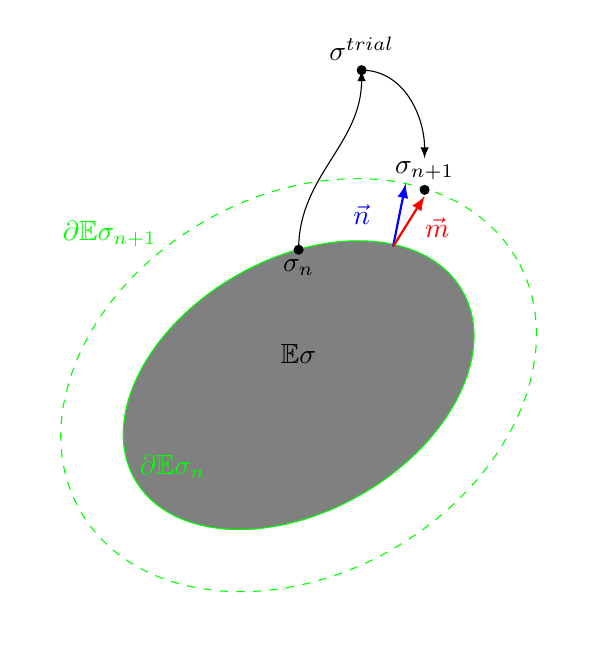
\begin{tikzpicture}[
  scale =0.8
]
  \filldraw[draw=green, fill=gray, rotate=30] (0,0) ellipse (3cm and 2cm);
  \draw[dashed, color=green, rotate=30] (0,0) ellipse (4cm and 3cm);
  \node at (0,0.5) {$\mathbb{E}\sigma$};
  \node[green] at (-2,-1.3) {$\partial \mathbb{E}\sigma_{n}$};
  \node[green] at (-3,2.4) {$\partial \mathbb{E}\sigma_{n+1}$};
  \filldraw[black] (0,2.15) circle (2pt) node[anchor=north] {$\sigma_{n}$};
  \draw[-latex] (0,2.15) to[out=90, in=270] (1, 5);
  \filldraw[black] (1,5) circle (2pt) node[anchor=south] {$\sigma^{trial}$};
  \filldraw[black] (2,3.1) circle (2pt) node[anchor=south] {$\sigma_{n+1}$};
  \draw[-latex] (1,5) to[out=0, in=90] (2, 3.6);
  % N
  \draw[-latex, blue, thick] (1.5,2.2) -- (1.7,3.2);
  \node[blue] at (1, 2.7) {$\vec{n}$};
  % M
  \draw[-latex, red, thick] (1.5,2.2) -- (2,3);
  \node[red] at (2.2, 2.5) {$\vec{m}$};

\end{tikzpicture}
\caption{Return mapping in 1D with strain hardening}
\label{fig:returnmap}
\end{figure}


\subsection{Rate-Independent Plasticity}
\label{Rate-Independent Plasticity}
Rate-independence means that what ever the rate the material is deformed, properties do not change because of it. This however, does not mean that material cannot undergo strain hardening. In this case, it is quite straightforward to obtain the increment of plastic strain. For the sake of simplicity and stay in line with the mock paper objectives, only 1D case will be defined.

From equation \ref{eq::kkt3},  
\begin{itemize}
  \item Key equation: $\Delta \lambda = f^{trial} / E$
\end{itemize}

\subsection{Viscoplasticity}
\label{Viscoplasticity}
In some cases and conditions, metals exhibit viscoplastic behavior. Viscoplasticity can be defined by the dependence of meterial state evolution to the strain rate. 
\begin{itemize}
  \item Perzyna mode: $\dot{\varepsilon}^{vp}= \dfrac{1}{n} \left\langle  \dfrac{f}{\sigma^{y}} \right\rangle^{n} sign(\sigma)$
  \item Physical meaning of $\eta$ and n
  \item Limiting case $n \rightarrow 0$ (recovers rate indenpendence)
\end{itemize}

\section{Implementation}
\label{Implementation}

\subsection{Algorithm Structure}
\label{Algorithm Structure}
\begin{itemize}
  \item Elastic predictor
  \item Yield check
  \item Plastic corrector
  \item Figure
  \begin{itemize}
    \item Simple flowchart to illustrate the process of return mapping
  \end{itemize}
\end{itemize}

\subsection{Code Organization}
\label{Code Organization}

\begin{algorithm}
\DontPrintSemicolon % Some LaTeX compilers require you to use \dontprintsemicolon instead
\KwIn{Current step material data ($\sigma_{n}, \varepsilon_{n}, \varepsilon^{p}_{n}$)}
\KwOut{Updated material data ($\sigma_{n+1}, \varepsilon_{n+1}, \varepsilon^{p}_{n+1}$)}
$max \gets a_1$\;
\For{$i \gets 2$ \textbf{to} $n$} {
  \If{$a_i > max$} {
    $max \gets a_i$\;
  }
}
\Return{$max$}\;
\caption{{\sc Max} finds the maximum number}\label{alg:one}
\label{algo:max}
\end{algorithm}


%% The Appendices part is started with the command \appendix;
%% appendix sections are then done as normal sections
\appendix
\section{Example Appendix Section}
\label{app1}

Appendix text.

%% Refer following link for more details.
%% https://en.wikibooks.org/wiki/LaTeX/Mathematics
%% https://en.wikibooks.org/wiki/LaTeX/Advanced_Mathematics

%% Use a table environment to create tables.
%% Refer following link for more details.
%% https://en.wikibooks.org/wiki/LaTeX/Tables
\begin{table}[t]%% placement specifier
%% Use tabular environment to tag the tabular data.
%% https://en.wikibooks.org/wiki/LaTeX/Tables#The_tabular_environment
\centering%% For centre alignment of tabular.
\begin{tabular}{l c r}%% Table column specifiers
%% Tabular cells are separated by &
  1 & 2 & 3 \\ %% A tabular row ends with \\
  4 & 5 & 6 \\
  7 & 8 & 9 \\
\end{tabular}
%% Use \caption command for table caption and label.
\caption{Table Caption}\label{fig1}
\end{table}

%% If you have bib database file and want bibtex to generate the
%% bibitems, please use
%%
\bibliographystyle{elsarticle-num} 
\bibliography{references}


\end{document}









%% Use \subsubsection, \paragraph, \subparagraph commands to 
%% start 3rd, 4th and 5th level sections.
%% Refer following link for more details.
%% https://en.wikibooks.org/wiki/LaTeX/Document_Structure#Sectioning_commands

\subsubsection{Mathematics}
%% Inline mathematics is tagged between $ symbols.
This is an example for the symbol $\alpha$ tagged as inline mathematics.

%% Displayed equations can be tagged using various environments. 
%% Single line equations can be tagged using the equation environment.
\begin{equation}
f(x) = (x+a)(x+b)
\end{equation}

%% Unnumbered equations are tagged using starred versions of the environment.
%% amsmath package needs to be loaded for the starred version of equation environment.
\begin{equation*}
f(x) = (x+a)(x+b)
\end{equation*}

%% align or eqnarray environments can be used for multi line equations.
%% & is used to mark alignment points in equations.
%% \\ is used to end a row in a multiline equation.
\begin{align}
 f(x) &= (x+a)(x+b) \\
      &= x^2 + (a+b)x + ab
\end{align}

\begin{eqnarray}
 f(x) &=& (x+a)(x+b) \nonumber\\ %% If equation numbering is not needed for a row use \nonumber.
      &=& x^2 + (a+b)x + ab
\end{eqnarray}

%% Unnumbered versions of align and eqnarray
\begin{align*}
 f(x) &= (x+a)(x+b) \\
      &= x^2 + (a+b)x + ab
\end{align*}

\begin{eqnarray*}
 f(x)&=& (x+a)(x+b) \\
     &=& x^2 + (a+b)x + ab
\end{eqnarray*}




% %% Use figure environment to create figures
% %% Refer following link for more details.
% %% https://en.wikibooks.org/wiki/LaTeX/Floats,_Figures_and_Captions
% \begin{figure}[t]%% placement specifier
% %% Use \includegraphics command to insert graphic files. Place graphics files in 
% %% working directory.
% \centering%% For centre alignment of image.
% \includegraphics{example-image-a}
% %% Use \caption command for figure caption and label.
% \caption{Figure Caption}\label{fig1}
% %% https://en.wikibooks.org/wiki/LaTeX/Importing_Graphics#Importing_external_graphics
% \end{figure}



%% For citations use: 
%%       \cite{<label>} ==> [1]

%%
Example citation, See \cite{lamport94}.



%% else use the following coding to input the bibitems directly in the
%% TeX file.

%% Refer following link for more details about bibliography and citations.
%% https://en.wikibooks.org/wiki/LaTeX/Bibliography_Management


\end{document}

\endinput
%%
%% End of file `elsarticle-template-num.tex'.
